% This is samplepaper.tex, a sample chapter demonstrating the
% LLNCS macro package for Springer Computer Science proceedings;
% Version 2.21 of 2022/01/12
%
\documentclass[runningheads]{llncs}
%
\usepackage[T1]{fontenc}
\usepackage{graphicx}
\usepackage{amsmath}
\usepackage{tikz}
\usetikzlibrary{arrows.meta,positioning,fit,backgrounds}
%
\begin{document}
%
\title{Evaluating and Improving Similarity-Aware Train-Test Splitting for Wildlife Re-Identification}
%
\titlerunning{Similarity-Aware Train-Test Splitting for Wildlife Re-Identification}
%
\author{Tshephang Matlala \inst{1} \and
Kamohelo Lebjane \inst{1} \and
Mogaladi Brilliant\inst{1}}
%
\authorrunning{T. Matlala et al.}
%
\institute{Academy of Computer Science and Software Engineering, University of Johannesburg, Johannesburg, South Africa}
%
\maketitle              % typeset the header of the contribution
%
\begin{abstract}
Re-identifying an individual animal from an image is a task that remains difficult even for
people, since two photographs of the same animal can look different depending on when, where,
and under what lighting they were taken. The WildlifeReID-10k dataset was introduced to push
research beyond simple species classification and towards the harder problem of individual
re-identification, and its main contribution is a splitting methodology, a time-aware split where
timestamps are available, and a similarity-aware split otherwise, that groups near-duplicate
images together using single-linkage clustering on DINOv2 features and keeps whole groups on one
side of the training/testing boundary. In this proposal we examine this splitting methodology in
detail, including a documented revision to the algorithm between the dataset's preprint and its
peer-reviewed camera-ready version, and identify several open questions worth investigating: how
much the similarity-aware split actually recovers of the leakage-correction effect that the
time-aware split achieves on datasets where both can be compared directly, whether the clustering
step is vulnerable to the well-known chaining effect of single-linkage clustering, and whether the
manually-chosen, per-dataset similarity threshold at its core can be replaced with something more
principled and reproducible. We lay out both these problems and a concrete plan for investigating
them.

\keywords{Animal re-identification \and Wildlife re-identification \and WildlifeReID-10k
        \and Clustering \and Single-linkage clustering \and Self-supervised learning \and DINOv2.}
\end{abstract}
%
%
%
\section{Introduction}

Re-identification is the task of deciding whether two images show the same individual. For
animals, this is a task that is difficult even for a person doing it by hand: telling apart two
photographs of lions, for instance, is not simply a matter of skill, since the two photographs
may have been taken at different times, in different locations, and under different lighting
conditions, and any of these differences alone can make the same individual look like a
different one. This is a fundamentally different problem from the one that datasets, such as
ImageNet were built to address. ImageNet and similar datasets were built around classification
and object detection, where the goal is to say \emph{what} is in an image (a lion, a bird, a
turtle). Re-identification instead asks \emph{which} individual is in the image, so it requires a
model to pick up on fine, individual specific detail rather than species level or category level
detail.

Beyond the difficulty of the task itself, being able to re-identify individual animals matters
because it is what makes long-term animal tracking possible. If a specific individual can be
recognised again in a later photograph, weeks or months after it was first seen, then it becomes
possible to follow what has happened to that animal over time, which would otherwise require
much more labour-intensive manual tracking~\cite{cermak2024wildfusion}. A concrete example of why
this is useful: a conservationist who treats a sick or injured wild animal with medication wants
to know afterwards whether the treatment actually worked, which means being able to find and
recognise that same individual again in later camera-trap or survey images, rather than only
being able to say that "some animal of this species" was seen again. The same reasoning applies to monitoring
population size, tracking migration, and studying how individual animals respond to
environmental change, all of which depend on reliably matching individuals across images taken at
different times, and this is precisely why re-identification, rather than only classification, is
the task that needs to be solved well.

The WildlifeReID-10k dataset~\cite{adam2025wildlifereid} was introduced specifically to support
this individual level task. In its peer-reviewed camera-ready form, it aggregates 37 existing
wildlife re-identification datasets into a single, cleaned collection of 140,488 images of 10,772
individuals across around 33 species, at a total size of only 26GB.\footnote{We note this
explicitly because the dataset has a documented revision history that matters for this proposal:
an earlier, June 2024 arXiv preprint of the same
paper~\cite{adam2024wildlifereidarxiv} described a collection of 30 datasets (214,262 images) and
used a different clustering algorithm for its splitting step, namely DBSCAN with a fixed maximal
cluster size of 5. Between that preprint and the CVPR Workshop 2025 camera-ready
version~\cite{adam2025wildlifereid} we cite throughout this proposal, the authors revised the
splitting algorithm to the single-linkage clustering method with a manually-set per-dataset
threshold described below. We treat this revision itself as relevant evidence: the fact that the
authors moved away from their original DBSCAN-based approach suggests they encountered
limitations with it worth understanding, even though our own investigation targets the current,
published algorithm.} Beyond aggregation, its central methodological contribution is a way of
splitting the data into training and testing sets that tries to avoid an easy trap: because many
images come from the same encounter, the same camera session, or even the same video, a naive
random split can place near-duplicate images on both sides of the split, which makes the
re-identification task look artificially easy and inflates reported performance. WildlifeReID-10k's
proposed fix has three steps. First, around 5\% of identities in each dataset are set aside
entirely for open-set testing. Second, for the remaining identities, a \emph{time-aware split} is
used wherever reliable timestamps are available: the oldest roughly 85\% of an individual's images
go to training and the rest to testing, guaranteeing that images from the same encounter cannot
end up on both sides. Third, since only 13 of the 37 constituent datasets have timestamps at
all,\footnote{Of these 13, the paper itself excludes 4 (AmvrakikosTurtles, ReunionTurtles,
StripeSpotter, ZakynthosTurtles) from its own time-aware split comparison due to too few images
or encounters, so the head-to-head evaluation we build on in P4 (Table 6 and Figure 5 of the paper)
actually compares 9 timestamped datasets against the remaining 28 without timestamps, not 13
against 24. We use ``13 timestamped datasets'' loosely throughout this proposal to mean the set of
datasets where timestamp metadata exists at all, and are precise about the smaller working set of 9
wherever we describe experiments that reproduce or extend the paper's own time-aware comparison.}
a \emph{similarity-aware split} is used everywhere else: images are embedded using
DINOv2~\cite{oquab2023dinov2}, and for each identity, a graph is built where an edge connects two
images if their cosine similarity exceeds a threshold $\theta$; the connected components of this
graph (found using a Union-Find/disjoint-set structure, i.e.\ single-linkage clustering) become the
clusters, and whole clusters are assigned to the training set, while the remaining, unclustered
images are split between training and testing.

The fact that images come from many different sources also affects re-identification directly: some
animals are photographed in the wild, under uncontrolled ground and background conditions, while
others are photographed in controlled environments, such as zoos or rehabilitation
centres~\cite{akbar2025body}. Because re-identification tends to be easier under controlled
conditions, this difference in image source is itself a factor that any evaluation of the
splitting methodology needs to account for.

In this proposal, our interest is specifically in this splitting methodology, and in particular in
the similarity-aware split, since it is the one applied to the large majority of the dataset's
constituent sources. We set out below the problems we see with the current approach, review the
related work that informs our proposed investigation, and describe the approach we intend to take.

\section{Problem Description}

Our research is organised around four research questions, moving from whether the current
similarity-aware split works, to whether it can be improved, to whether that improvement
generalises and matters downstream:

\begin{quote}
\emph{RQ1.} How effectively does the similarity-aware split prevent train-test leakage, compared
with the time-aware split, on the datasets where both can be computed and compared directly?

\emph{RQ2.} Can alternative threshold-selection and clustering strategies improve the reliability
of the similarity-aware split relative to the current manually-tuned single-linkage method?

\emph{RQ3.} Does a split methodology developed and validated on the 13 timestamped datasets
remain reliable when deployed on the 24 datasets that have no timestamps to validate it against?

\emph{RQ4.} How do improvements in split reliability, and training-time data augmentation applied
within the resulting splits, affect downstream open-set and closed-set wildlife re-identification
performance?
\end{quote}

These four questions correspond to four hypotheses we intend to test:

\begin{quote}
\emph{H1.} The current similarity-aware split does not fully reproduce the leakage-correction
effect that the time-aware split achieves on the same, timestamped datasets.

\emph{H2.} Single-linkage clustering produces chained clusters containing image pairs whose
direct pairwise similarity falls substantially below the clustering threshold $\theta$.

\emph{H3.} Automatic threshold selection and/or chain-resistant clustering methods produce higher
cluster quality, measured against timestamp agreement, than the current manually-tuned
single-linkage method.

\emph{H4.} Split-quality improvements validated on the 13 timestamped datasets, together with
training-only data augmentation, produce more reliable downstream Re-ID evaluation once deployed
across the full, heterogeneous WildlifeReID-10k collection.
\end{quote}

We break this down into seven concrete problems with the current methodology, grouped under the
three limitations these hypotheses target: threshold selection (P1), clustering robustness (P2,
P3), and validation/generalisation (P4, P5), plus two supporting concerns, imbalance (P6) and
per-dataset heterogeneity (P7), that we treat as secondary to the central splitting problem.

Before setting out these seven problems, we want to be precise about what we mean by ``leakage,''
since the term is used loosely in the paper and conflating its senses would weaken our own
experimental claims. We distinguish three related but distinct notions: \emph{image-level} leakage,
where near-identical images (for instance, consecutive video frames) appear on both sides of the
split; \emph{encounter-level} leakage, where images from the same observation event appear on both
sides even if no two images are near-duplicates; and \emph{identity-level} leakage, where the same
individual appears in both training and testing. These are not interchangeable. In closed-set
re-identification, identity-level overlap between train and test is expected and necessary, since
the task is precisely to recognise known individuals again; it is not leakage in the harmful sense.
Image- and encounter-level leakage, however, can make the benchmark artificially easy regardless of
the evaluation protocol, because the model may be relying on incidental cues (the same background,
the same lighting, the same pose) rather than on identity-discriminative features.
WildlifeReID-10k's splitting methodology is aimed squarely at removing image- and encounter-level
leakage, and this is the sense in which we use the term throughout this proposal unless stated
otherwise.

Relatedly, we adopt the following formal distinction between the two evaluation protocols the
paper (and our proposal) reports results under. In the \emph{closed-set} protocol, every identity
that appears in the test set also appears in the training set, $ID_{\text{test}} \subseteq
ID_{\text{train}}$, and the model's task is to identify the individual among a fixed set of known
identities. In the \emph{open-set} protocol, some test identities are deliberately withheld from
training, $ID_{\text{test}} \not\subseteq ID_{\text{train}}$, and the model must additionally
decide whether a query corresponds to a known identity at all, rather than being forced to pick the
closest match among known individuals. Open-set evaluation is precisely where correct split
construction matters most, since if a withheld identity's images leak into training through an
image- or encounter-level near-duplicate, the identity is no longer genuinely unseen, and the
open-set protocol silently degrades back into a closed-set one for that individual.

P1: the similarity threshold is manually chosen, and this is only validated on a small,
favourable subset of the data. WildlifeReID-10k's clustering step depends entirely on a cosine
similarity threshold $\theta$ that decides which images count as near-duplicates. The paper
reports that a single global threshold ($\theta = 0.97$) found 5,601 true-positive duplicate pairs
against 685 false positives on the datasets with timestamps, but that manually choosing a
different threshold for each dataset, based on visual inspection, improved this substantially, to
8,206 true positives against only 464 false positives, and this manual, per-dataset approach is
what was actually used for the datasets without timestamps. This raises two separate concerns.
First, "based on visual inspection" is not a documented, repeatable procedure; different people
inspecting the same clusters could plausibly choose different thresholds, and the paper does not
report what values were chosen for which datasets or how sensitive the results are to that choice.
Second, and more importantly, this manual tuning is only checked against ground truth on the 13
datasets that have timestamps. For the remaining 24 datasets, which have no timestamps at all,
there is no way, even in principle, to verify whether the manually-chosen threshold is any good,
since there is no ground truth to compare it against. The manual method's advantage over the
single global threshold is demonstrated only where it can be checked, and then applied on faith
everywhere else.

P2: single-linkage clustering is structurally vulnerable to the chaining effect. The clustering
step is not, in fact, DBSCAN, as an earlier preprint of this paper described; it is single-linkage
clustering, implemented via connected components over a similarity graph. This is a different
algorithm with a different, well-documented weakness. Single-linkage clustering builds clusters by
transitively connecting any two points reachable through a chain of pairwise similarities above
the threshold, so if image A is similar enough to image B, and image B is similar enough to image
C, then A and C are placed in the same cluster even if A and C are not similar to each other at
all. This is a long-recognised limitation of single-linkage clustering in the general clustering
literature, commonly called the chaining effect~\cite{jain1999data}. In the context of
WildlifeReID-10k, this matters because a long, gradually-changing sequence of images from a single
encounter (an animal slowly turning, walking away, or moving in and out of shadow) is exactly the
kind of chain that could merge visually very different images of the same individual into one
oversized cluster, an outcome that could quietly inflate the size of the training-only cluster
bucket well beyond genuine near-duplicates, without ever being flagged as a false positive under
the paper's own quality metric, since that metric only checks whether a cluster's images share the
same timestamp, not whether every pair of images inside the cluster is actually similar to every
other pair.

P3: the cluster assignment is still a hard, binary decision. Despite the change in the underlying
clustering algorithm, the fundamental character of the decision it produces has not changed: an
image either belongs to a cluster or it does not, with no accompanying measure of confidence. The
paper's own Table 3 shows that cluster purity (the share of a cluster's images sharing a single
timestamp) degrades as clusters grow larger, from 97.5\% for clusters of size 2 down to 77.4\% for
clusters of size 6 or more, which means that for the largest clusters, roughly one in five images
placed inside them may not actually belong to the same encounter as the rest, yet every image
inside the cluster is treated identically once it is assigned.

P4: the similarity-aware split recovers far less of the leakage-correction effect than the
time-aware split does, on the paper's own evidence. This is, in our view, the most important open
question raised by the paper's own results. The paper's Table 6 reports performance on the
MiewID foundation model under four conditions: on the datasets that have timestamps, moving from a random
split to a time-aware split closes a 12.3-point gap in closed-set accuracy (81.5\% to 69.2\%) and a
16.7-point gap in open-set performance (72.6\% to 55.9\%). But on the datasets without timestamps,
moving from a random split to the similarity-aware split closes only a 1.5-point gap in closed-set
accuracy (80.8\% to 79.3\%) and a 2.5-point gap in open-set performance (66.1\% to 63.6\%). The
paper's own introduction explicitly frames the similarity-aware split as an extension of the
time-aware split, meant to approximate its effect when timestamps are unavailable. If that is the
intended relationship, this gap is difficult to reconcile: the similarity-aware split therefore
appears to recover substantially less of the performance correction observed under the time-aware
split. This could mean that the similarity-aware split is only catching a small fraction
of genuine same-encounter leakage, or it could mean that the underlying datasets without
timestamps are simply different in other ways, but the paper's experiments do not separate these
two explanations, since split type and dataset group always co-vary in this comparison.

P5: cluster quality can only be checked where it is least needed. The paper's true-positive/
false-positive validation framework (Section 3.3 of the paper) can only be computed on datasets
that have timestamps, because it needs a timestamp to check whether a cluster's images were really
taken together. This means cluster quality is verified only on the 13 datasets that already have a
better option available to them, the time-aware split, while the 24 datasets that actually depend
on the similarity-aware split for their entire leakage protection have no way of confirming that
their clusters are any good.

P6: the dataset is heavily imbalanced, and this is entangled with the wild-versus-controlled
question. WildlifeReID-10k is heavily imbalanced across species and individuals, for example
roughly 52,000 bird images spread across only 50 individuals against roughly 21,500 sea turtle
images spread across 2,703 individuals, and this imbalance is not evenly distributed by capture
condition either: about 50\% of individuals in the dataset were observed in the wild (71\%
including rehabilitation centres), and re-identification tends to be noticeably easier in
controlled, good-lighting conditions than it is in the wild, which the paper's own per-dataset
results reflect, since the best-performing datasets are mostly from controlled environments and
the worst-performing ones are mostly from the wild. This raises a question we want to investigate
directly: can data augmentation be used to help balance the dataset, so that species and
individuals with very few images are not simply left underrepresented, and does augmentation
narrow the gap between wild and controlled-environment performance, or does it mainly help the
already better-performing controlled-environment datasets.

P7: aggregate metrics can hide how differently a method performs across the 37 source datasets.
WildlifeReID-10k is a combination of 37 separate constituent datasets, each collected with a
different camera, at a different image resolution, and under different environmental conditions,
and each contributing very different numbers of images and individuals to the whole. The paper
does report a per-dataset breakdown of BAKS for its baseline models (its Figure 4), which is a good
existing practice, but this breakdown is not extended to the clustering step itself: we do not know
whether the similarity-aware split's clusters are good on some source datasets and poor on others,
only that the aggregate 76.1\%-style purity figures (now the Table 3 purity breakdown) hold
\emph{averaged} over the 13 timestamped datasets. We are therefore interested in extending this
per-dataset lens specifically to cluster quality, not just to downstream model performance.

\section{Related Work}

\emph{Self-supervised vision transformers (DINO and DINOv2).} The clustering step used to build
the similarity-aware split depends entirely on the quality of the image features it clusters, so
the feature extractor itself is directly relevant related work, and it is important to keep two
different papers distinct here. DINO~\cite{caron2021emerging} (2021) introduced a self-distillation
approach for training vision transformers with no labels at all: a student network learns to match
the representations a teacher network produces for a different augmented view of the same image,
rather than being trained with human-provided labels; the teacher shares the student's architecture
but is never updated by gradient descent, instead tracking an exponential moving average of the
student's weights, and collapse (both networks trivially agreeing on a constant output) is avoided
through centering and sharpening rather than any contrastive loss. This is self-distillation in
DINO's specific sense, a student matching a teacher's representations under augmentation, and
should not be confused with conventional knowledge distillation, which transfers a large model's
predictions into a smaller model. The property of DINO that matters most for our proposal is that
its self-supervised features cluster visually similar images together well, and its attention maps
naturally highlight object regions without ever being told to. DINOv2~\cite{oquab2023dinov2}
(2023) is DINO's larger, later successor: it scales the same self-distillation idea to a bigger
curated dataset and model size and produces stronger, more general-purpose visual features. It is
specifically DINOv2, not the original DINO, whose embeddings WildlifeReID-10k uses to build its
similarity graph, and DINOv2 features are also what the paper uses directly as one of the tools to
sanity-check the quality of the clustering itself.

\emph{Face re-identification (SurvFace).} Cheng et al.~\cite{cheng2020face} study a closely
related re-identification problem in a different domain, introducing SurvFace, a benchmark for
face re-identification built by mining face crops out of 17 existing person re-identification
datasets rather than collecting new data. The paper draws a distinction that maps directly onto
our own problem: standard face recognition models are trained and tested on clean, cooperative,
high-resolution web photographs, while surveillance-style face re-identification must work with
uncontrolled, low-resolution, poorly lit images, and models trained only on the former generalise
surprisingly poorly to the latter. SurvFace also uses the same closed-set/open-set distinction that
WildlifeReID-10k uses, and its metrics (FPIR, FNIR, TPIR@FPIR for open-set; CMC and rank-1 for
closed-set) are not directly reused in WildlifeReID-10k. This is not because they would be
technically inapplicable to animals, but because they assume a small watch-list style search and
do not correct for severe class imbalance, whereas WildlifeReID-10k's BAKS/BAUS metrics were
designed specifically to handle the extreme imbalance present in wildlife data. This is a useful,
concrete illustration of a point that recurs throughout this proposal: the choice of evaluation
metric should follow the shape of the underlying data.

\emph{Clustering-based pseudo-labelling and hard cluster assignment (Person Re-ID survey).}
Kumar et al.~\cite{personreidsurvey} survey supervised and unsupervised techniques for person
re-identification, a problem that is structurally the same as animal re-identification: given a
query image, retrieve the matching identity from a gallery of candidates. Two parts of this survey
are particularly relevant to our proposal. First, unsupervised domain adaptation methods generate
pseudo-labels through clustering algorithms such as DBSCAN or $k$-means, which confirms that
clustering-based pseudo-labelling in general, not any one specific algorithm, is a standard tool
across this wider literature. Second, and more directly relevant to WildlifeReID-10k's current
algorithm, this survey identifies noisy pseudo-labels as a general weakness of hard,
clustering-based assignment, arising both from domain gaps between source and target data and from
the coarse, all-or-nothing nature of the assignment itself, regardless of which clustering
algorithm produces it. Soft pseudo-labelling, where a probability of cluster membership is used
instead of a binary in/out label, is proposed in this literature as the fix, and this remains a
nuance that WildlifeReID-10k's current single-linkage clustering step does not explore, since
connected components are, by construction, a hard partition.

\emph{Chaining effect and alternatives to single-linkage clustering.} The specific weakness we
raise in P2, that single-linkage clustering (which is what WildlifeReID-10k's connected-components
procedure implements) is prone to transitively merging dissimilar points through an unbroken chain
of intermediate similarities, is a long-established result in the clustering literature, going back
to early critiques of the method and surveyed in general terms by Jain et
al.~\cite{jain1999data}. A variety of fixes have been proposed for this specific weakness over the
years, most of them built around the idea of using local density to break spurious chains before
they can form, filtering out low-density bridging points before running single-linkage, rather than
using the raw similarity graph directly. This body of work is directly relevant to our proposed
approach below, since density-adaptive clustering methods such as
HDBSCAN~\cite{campello2013density,campello2015hierarchical} were developed partly to address this
exact failure mode in a principled way.

\emph{Automatic threshold and cluster-count selection.} The manual, per-dataset threshold
tuning we raise in P1 has a long-standing automatic alternative in the general clustering
literature: the silhouette score~\cite{rousseeuw1987silhouettes}, which measures, for each point,
how much more similar it is to its own cluster than to the next closest cluster, and can be
averaged across all points to score a candidate clustering without needing any ground-truth labels.
Because it requires no labels, it is exactly the kind of automatic criterion that could replace
visual inspection when choosing $\theta$ per dataset, and it is widely used elsewhere for this
purpose in unsupervised settings where, as in WildlifeReID-10k's 24 datasets without timestamps,
no ground truth is available to validate the choice directly.

\emph{Transformer-based re-identification and animal re-identification benchmarks.} Ye et
al.~\cite{ye2025transformer} provide a transformer-era follow-up to the Person Re-ID survey above,
and its Animal Re-ID section is the most directly relevant part of the related work to our
proposal. This section confirms that animal re-identification, as a field, is still immature
compared to person or vehicle re-identification, with unclear task boundaries, species-specific
methods that do not transfer well across species, and inconsistent experimental protocols across
papers, which is essentially the same gap that motivated WildlifeReID-10k's own creation. In the
same section, the authors also confirm that clustering-based pseudo-labelling remains the default
approach for unsupervised re-identification even in transformer-based pipelines, which reinforces
that the general weaknesses of hard, clustering-based assignment we describe above are a live,
general methodological gap rather than something specific to wildlife data.

\emph{Open-set evaluation under class imbalance.} Mendes J\'unior et al.~\cite{mendes2017open}
propose an open-set classifier together with normalized accuracy and open-set F-measure, evaluation
criteria designed to remain meaningful when the number of examples per class is highly uneven.
BAKS and BAUS, the two metrics WildlifeReID-10k reports throughout, are themselves built on this
line of work, which matters for our proposal because every one of our proposed experiments (P1--P7)
is run over a collection whose constituent datasets vary by orders of magnitude in size and where
naively-averaged accuracy would be dominated by whichever few datasets happen to be largest.


\section{Proposed Approach}

Our proposed approach is a single pipeline, applied identically to all 37 constituent datasets:
images are optionally augmented, embedded with DINOv2, compared via cosine similarity, clustered,
and split into training and testing sets. Timestamp availability plays no role in this pipeline
itself; the same augmentation, feature extraction, similarity, and clustering steps run regardless
of whether a given dataset happens to have timestamps. Timestamps are used only afterward, as a
validation signal: for the subset of datasets where timestamps exist, we can check the resulting
clusters against them to see whether the pipeline is behaving sensibly, in the same way the
original paper does. This keeps the method itself general-purpose and deployable everywhere, while
still letting us sanity-check it wherever a check happens to be possible.

Figure~\ref{fig:pipeline} summarises this pipeline. It is a single, linear sequence of six steps,
augmentation, DINOv2 feature extraction, similarity comparison, clustering, splitting, and
evaluation, run the same way for all 37 datasets. Timestamp checking is not one of these six steps.
It is a separate validation check, shown below the main sequence in the figure, that we apply
afterwards to see how well the clustering step worked, and only where timestamps happen to exist.

\begin{figure}[t]
\centering
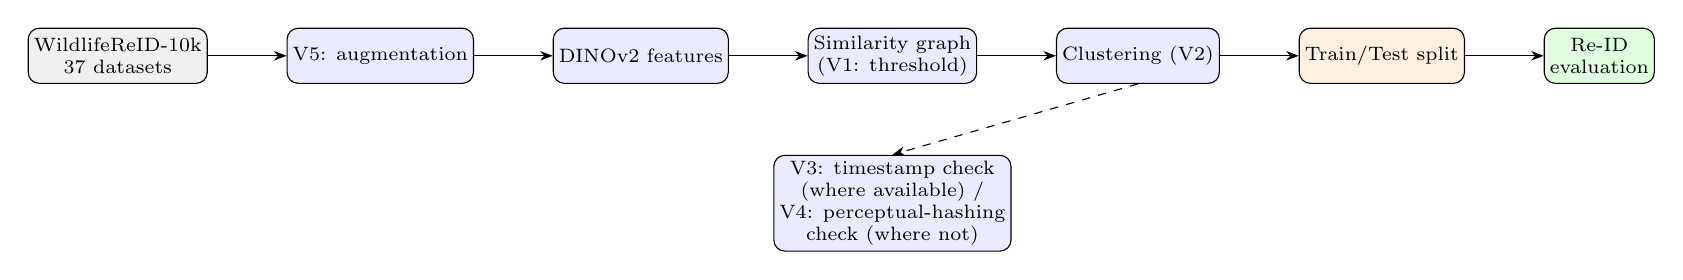
\begin{tikzpicture}[
  node distance=8mm and 10mm,
  box/.style={draw, rounded corners, align=center, minimum height=7mm, inner sep=2pt, font=\scriptsize},
  data/.style={box, fill=gray!12},
  pstage/.style={box, fill=blue!8},
  split/.style={box, fill=orange!12},
  eval/.style={box, fill=green!12},
  arr/.style={-{Stealth[length=1.6mm]}, thin}
]

\node[data] (raw) {WildlifeReID-10k\\37 datasets};
\node[pstage, right=of raw] (aug) {V5: augmentation};
\node[pstage, right=of aug] (dino) {DINOv2 features};
\node[pstage, right=of dino] (sim) {Similarity graph\\(V1: threshold)};
\node[pstage, right=of sim] (clust) {Clustering (V2)};
\node[split, right=of clust] (splitn) {Train/Test split};
\node[eval, right=of splitn] (reid) {Re-ID\\evaluation};

\node[pstage, below=9mm of sim] (valid) {V3: timestamp check\\(where available) /\\V4: perceptual-hashing\\check (where not)};

\draw[arr] (raw) -- (aug);
\draw[arr] (aug) -- (dino);
\draw[arr] (dino) -- (sim);
\draw[arr] (sim) -- (clust);
\draw[arr] (clust) -- (splitn);
\draw[arr] (splitn) -- (reid);

\draw[arr, dashed] (clust.south) -- (valid.north);

\end{tikzpicture}
\caption{Overview of the proposed pipeline. The same six steps, augmentation, DINOv2 feature
extraction, similarity estimation, clustering, splitting, and evaluation, run identically for all
37 constituent datasets, regardless of whether timestamps are available. The dashed arrow shows
validation applied afterward, as a check on the resulting clusters rather than a step in the
pipeline itself: timestamp agreement where timestamps exist (V3), and perceptual hashing as an
independent, model-free second opinion where they do not (V4).}
\label{fig:pipeline}
\end{figure}

\begin{itemize}
\item[\emph{V1}] Replace the manual, per-dataset threshold with an automatic one. For each
dataset, we sweep candidate values of $\theta$ and score the resulting clustering with the
silhouette score~\cite{rousseeuw1987silhouettes}, which needs no ground-truth labels, and select
the value that scores best. This directly targets P1 and H3: it removes the undocumented,
visual-inspection step from threshold choice, and, unlike manual tuning, gives us a criterion we
can also apply, and trust, on the 24 datasets that have no timestamps to check the threshold
against.
\item[\emph{V2}] Directly test whether the chaining effect is a real problem
in practice, not just a theoretical one, by running the current connected-components (i.e.\
single-linkage) clustering and a chain-resistant alternative, complete-linkage clustering, through
the same pipeline on every dataset. Complete-linkage only merges two points into the same cluster
if every pairwise similarity inside the resulting cluster stays at or above $\theta$, which directly
attacks chaining, since no chain of intermediate similarities can smuggle a dissimilar pair into a
cluster, while remaining a standard, well-understood algorithm rather than one we would need to
justify from scratch. Both variants are run identically across all 37 datasets, using the threshold
from V1; we then use whichever subset happens to have timestamps purely to check which variant
agrees better with timestamp agreement, without that check being part of the pipeline itself. We
will also report how often the current method's largest clusters (size 6+, where Table 3 shows
purity already drops to 77.4\%) contain image pairs whose direct pairwise similarity is far below
$\theta$, which would be direct evidence of chaining.
\item[\emph{V3}] On the subset of datasets that happen to have usable timestamps (9 of the 13
with timestamp metadata; see the footnote above), reproduce the comparison behind Table 6 as a
validation check on the pipeline's output: random split, time-aware split, the current
similarity-aware split, and our V2 alternative, all measured against each other on the same data.
This directly answers whether an improved clustering step closes more of the 12.3/16.7-point gap
that the current similarity-aware split only partially closes, without requiring the pipeline
itself to treat timestamped and non-timestamped datasets any differently.
\item[\emph{V4}] The pipeline's own timestamp-agreement check (V3) can only be computed where
timestamps exist. As a validation check on the pipeline's output for the datasets that lack them,
we use an independent, model-free signal instead: perceptual hashing, a long-standing technique
for near-duplicate detection unrelated to any learned embedding, and check where DINOv2-based
clusters and perceptual-hashing-based near-duplicate flags agree or disagree. Disagreements are
exactly the borderline cases worth flagging for extra scrutiny. We treat agreement between the two
as an independent, model-free near-duplicate detection signal that increases our confidence in a
cluster, not as proof that the cluster is correct: perceptual hashing can respond to shared
background, composition, or pose rather than to the animal itself, and conversely the same
individual photographed under very different conditions can hash very differently, so it is a
useful second opinion rather than a ground truth in its own right.
\item[\emph{V5}] Investigate whether controlled data augmentation, applied
\emph{before} DINOv2 feature extraction and similarity analysis rather than only during Re-ID
training, improves the robustness of the similarity representation used for clustering, with
particular attention to underrepresented species and individuals (for example sea turtles relative
to birds) and to wild-captured individuals relative to controlled-environment ones. Concretely, we
generate augmented views (flips, crops, brightness/lighting changes, rotation) of each image,
extract DINOv2 features for both the original and augmented views, and include the augmented views
in the similarity graph and clustering step itself, rather than adding them only after the
train/test split has already been fixed. This makes augmentation a controlled factor in the
similarity-analysis pipeline: we compare a no-augmentation baseline against an augmented condition,
with clustering, splitting, and downstream Re-ID training otherwise identical, and measure whether
augmentation changes cluster quality, split quality, and the balanced-accuracy gap between
well-represented and poorly-represented classes and between wild and controlled-environment
datasets, without simply inflating scores on the classes that are already well represented. We
define a reproducible, non-arbitrary criterion for which individuals count as low-resource (fewer
than a fixed threshold of training images) rather than hand-picking species after the fact.
\end{itemize}

As secondary, lower-priority directions that are already supported by the related work above but
are not our primary focus, we note the possibility of a rotation-invariant backbone for the
wild, uncontrolled-pose subset of the data, so that, for example, the same bear photographed once
on land and once in a river is still recognised as the same individual
regardless of background~\cite{vidal2021perspectives}; of wildlife-specific self-supervised
pretraining as an alternative to using generic off-the-shelf DINOv2 features; and of
dataset-aware clustering, which
would treat each of the 37 constituent datasets as its own visual domain so that shared per-source
style (lighting, background, camera setup) is not mistaken for true individual similarity.

\begin{credits}
\subsubsection{\ackname} This proposal is submitted as part of a group project undertaken at the
University of Johannesburg.

\subsubsection{\discintname}
The authors have no competing interests to declare that are relevant to the content of this
proposal.
\end{credits}
%
% ---- Bibliography ----
%
\bibliographystyle{splncs04}
\bibliography{references}

\end{document}